\section{Our Work}
In this section, we shall present our work. The code for the same can be found on Git hub\footnote{\url{https://github.com/Ankan-Mukherjee/NIUS.git}}. Our work essentially includes designing a suitable hash function and then cracking it using Generalized Grover Search algorithm. 
We are working on \textbf{8-bit hashes}. Note that we will use the \textbf{little-endian system} throughout, i.e., $S_0$ represents the Most Significant Bit and $S_7$ the Least Significant Bit.
\subsection{Classical Hashing Algorithm}
The hashing algorithm followed is the 8-bit Pearson Hash generation using 2 LFSRs. The taps for the first LFSR are at indices $3$, $4$, $5$ and $7$. The taps for the second LFSR are at indices $1$, $2$, $4$ and $7$. The diagrams for the same are presented in figures \ref{Fig:6.1} and \ref{Fig:6.2} respectively.
\begin{figure}[!htb]
   \begin{minipage}{\textwidth}
     \centering
     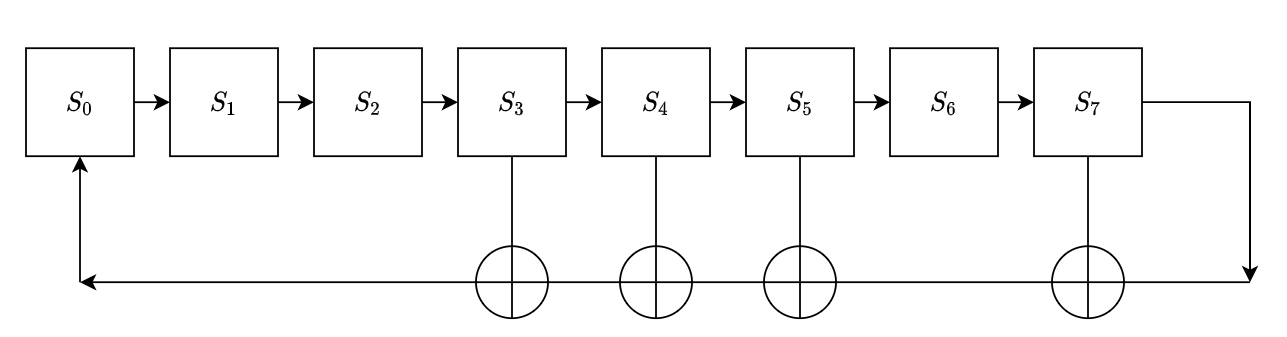
\includegraphics[width=\linewidth]{fig06.01.png}
     \caption{The First LFSR}
     \label{Fig:6.1}
   \end{minipage}
   \begin{minipage}{\textwidth}
     \centering
     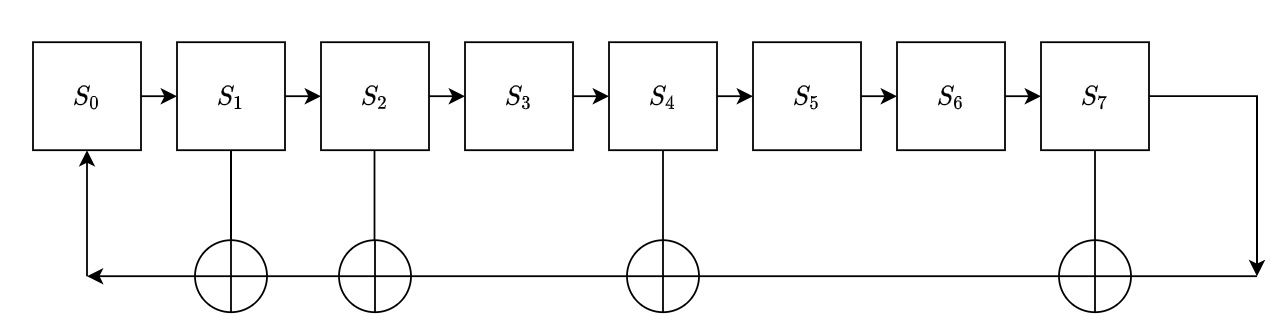
\includegraphics[width=\linewidth]{fig06.02.png}
     \caption{The Second LFSR}
     \label{Fig:6.2}
   \end{minipage}
\end{figure}
Characters are read from the message one at a time. The register is updates by taking its XOR with the ASCII of the character. The new value obtained is then passed through the first LFSR, followed by the second LFSR. The process is repeated for all characters till the end of the message. The code for the same is shown below.
\begin{lstlisting}
def LFSR1_Classical(x):
    bit = ((x >> 0) ^ (x >> 2) ^ (x >> 3) ^ (x >> 4)) & 1
    x = ((x >> 1)|(bit<<7))%256;
    return x
def LFSR2_Classical(x):
    bit = ((x >> 0) ^ (x >> 3) ^ (x >> 5) ^ (x >> 6)) & 1
    x = ((x >> 1)|(bit<<7))%256;
    return x
def hash_Classical(message):
    x=0
    for i in message:
        x=x^ord(i)
        x=LFSR1_Classical(x)
        x=LFSR2_Classical(x)
    return x

message=input().rstrip()
print(hash_Classical(message))
\end{lstlisting}
Now we shall check the values of the hash for some sample strings. This can be done by running the code given above.\\
Message: \verb|Hello World|\\
Hash: \verb|15|\\
Making a slight change\\
Message: \verb|Hello Workd|\\
Hash: \verb|239|\\
We see that the hash changes significantly.

\subsection{Quantum Hashing Algorithm}
Now we will implement the same hashing algorithm on a quantum computer. This will make use of one quantum register comprising $8$ qubits. The nonce itself will be stored on a register of 8 qubits. One qubit will be the output qubit that decides if a given hash is valid or not. Thus, our circuit will make use of $17$ qubits in total, along with some classical bits.  
\subsubsection*{The Two LFSRs and Their Inverses}
Let us first take a look at the two LFSR circuits, given in figures \ref{Fig:6.3} and \ref{Fig:6.4} respectively. These LFSRs perform the same function as the classical LFSRs, except that they do it on qubits.
\begin{figure}[!htb]
   \begin{minipage}{\textwidth}
     \centering
     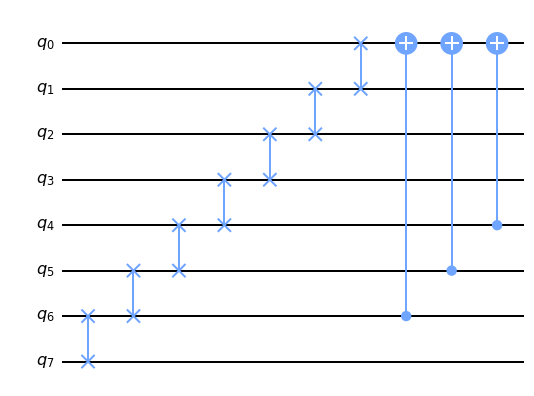
\includegraphics[width=0.9\linewidth]{fig06.03.png}
     \caption{The First LFSR}
     \label{Fig:6.3}
   \end{minipage}
   \begin{minipage}{\textwidth}
     \centering
     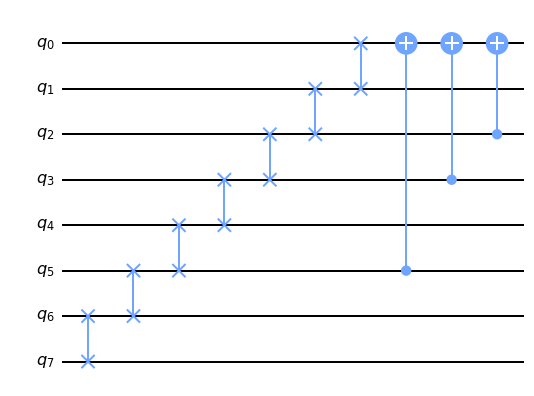
\includegraphics[width=0.9\linewidth]{fig06.04.png}
     \caption{The Second LFSR}
     \label{Fig:6.4}
   \end{minipage}
\end{figure}

For a quantum computer, it is imperative that after each iteration, the registers are restored to the original state for the next iteration to take place successfully. We need to design the circuits for inverting the LFSRs as well. These circuits are shown in figures \ref{Fig:6.5} and \ref{Fig:6.6} respectively.
\begin{figure}[!htb]
   \begin{minipage}{\textwidth}
     \centering
     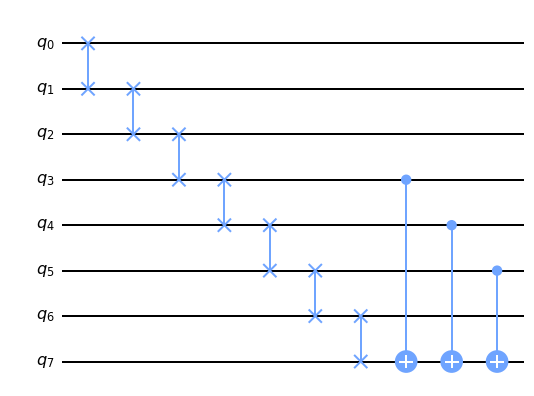
\includegraphics[width=0.9\linewidth]{fig06.05.png}
     \caption{Inverse of the First LFSR}
     \label{Fig:6.5}
   \end{minipage}
   \begin{minipage}{\textwidth}
     \centering
     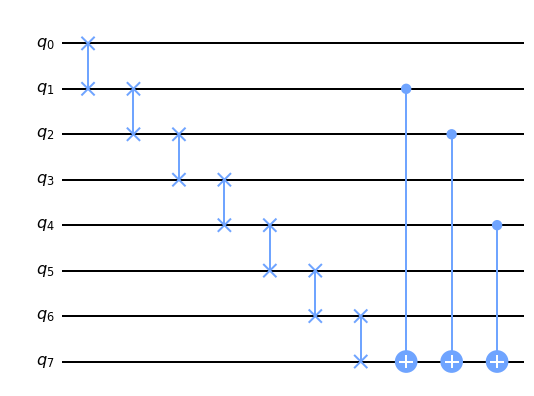
\includegraphics[width=0.9\linewidth]{fig06.06.png}
     \caption{Inverse of the Second LFSR}
     \label{Fig:6.6}
   \end{minipage}
\end{figure}

\subsubsection*{The Hashing Operation}
\noindent The hashing is performed in the following steps.
\begin{enumerate}
\item The classical algorithm is used to compute the hash till the end of the message block, just before the nonce.
\item The quantum hash register of $8$ qubits is initialized with the hash generated.
\item The nonce is XORed with the hash register using CX gates.
\item The first LFSR with taps at $3$, $4$, $5$ and $7$ is operated once on the hash register.
\item The second LFSR with taps at $1$, $2$, $4$ and $7$ is operated once on the hash register.
\end{enumerate}
The circuit for the entire hashing operator is shown in figure \ref{Fig:6.7}.
\begin{figure}[!htb]
   \begin{minipage}{\textwidth}
     \centering
     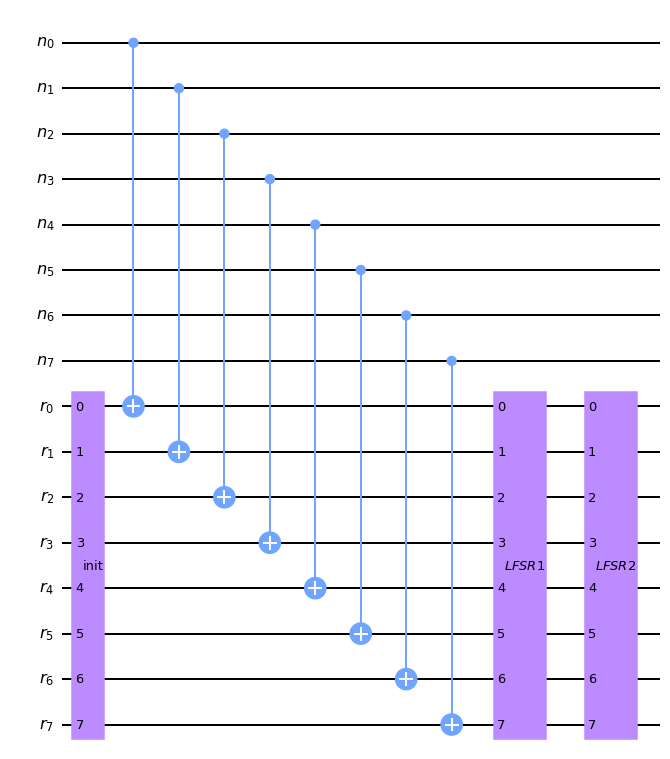
\includegraphics[width=0.8\linewidth]{fig06.07.png}
     \caption{Hashing Circuit}
     \label{Fig:6.7}
   \end{minipage}
\end{figure}

\subsubsection*{The Oracle}
It is now time to put everything together. We shall assume that a valid nonce is one that starts with $5$ zeroes. For this, we need to check if the registers at indices $0$, $1$, $2$, $3$ and $4$ are $\ket{0}$. A multi-controlled Toffoli gate from these register qubits to the output will flip the qubits of the output if and only if all of the $5$ qubits were $\ket{1}$. Further, if the output is initialized to $\ket{out}=\bfrac{\ket{0}-\ket{1}}{\sqrt{2}}$, we will get the output to flip sign only when all of the $5$ qubits are $\ket{1}$ or else output stays the same. Since we are interested in checking if all the $5$ qubits are $\ket{0}$, we must use $X$ gates on them before passing them through the multi-controlled Toffoli gate. After the check, we must restore the registers by inverting the operations applied. This invovles taking an $X$ gate on qubits $0$, $1$, $2$, $3$ and $4$, followed by the inverse of the second LFSR, followed by the inverse of the first LFSR. Figure \ref{Fig:6.8} shows the complete oracle circuit.
\begin{figure}[!htb]
   \begin{minipage}{\textwidth}
     \centering
     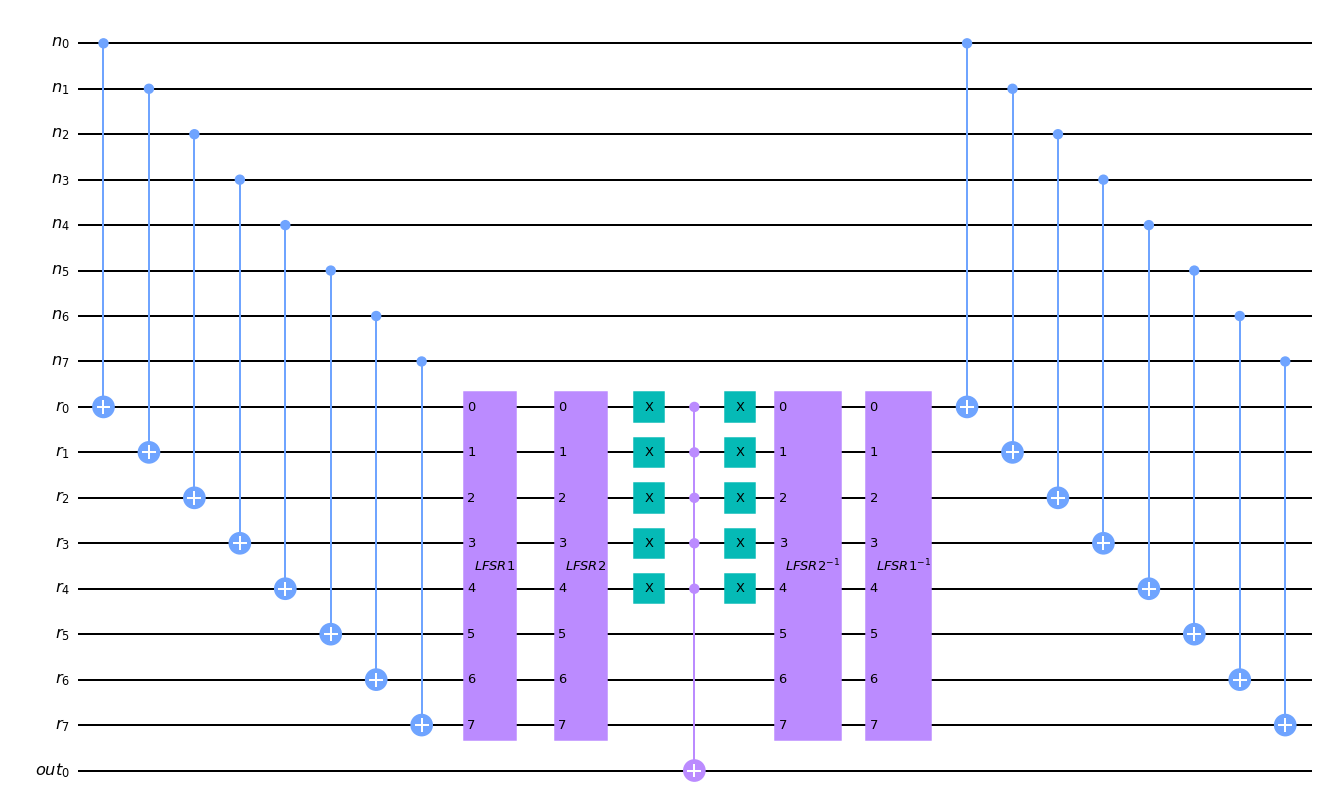
\includegraphics[width=\linewidth]{fig06.08.png}
     \caption{Circuit for the Oracle}
     \label{Fig:6.8}
   \end{minipage}
\end{figure}

\subsection{Searching the Nonce}

\subsubsection*{Grover Search}
The grover search involves setting up the nonce to a superposition of all states using a $H$ gate on all the qubits followed by the repeated application of the oracle followed by the diffuser. The diffuser used has been discussed in the section preceding figure \ref{Fig:5.3}. The number of iterations required is given by equation \ref{eq:5.9}, where, we now have $M=8$ solutions instead of $1$. Thus, number of iterations, $k$, is
\begin{equation}
\label{eq:6.1}
k=\left\lfloor\bfrac{\pi}{4}\sqrt{\bfrac{N}{M}}\right\rfloor=\left\lfloor\bfrac{\pi}{4}\sqrt{\bfrac{256}{8}}\right\rfloor=4
\end{equation}
Finally, we perform a measurement of the nonce. Figure \ref{Fig:6.9} shows the entire circuit.
\begin{figure}[!htb]
   \begin{minipage}{\textwidth}
     \centering
     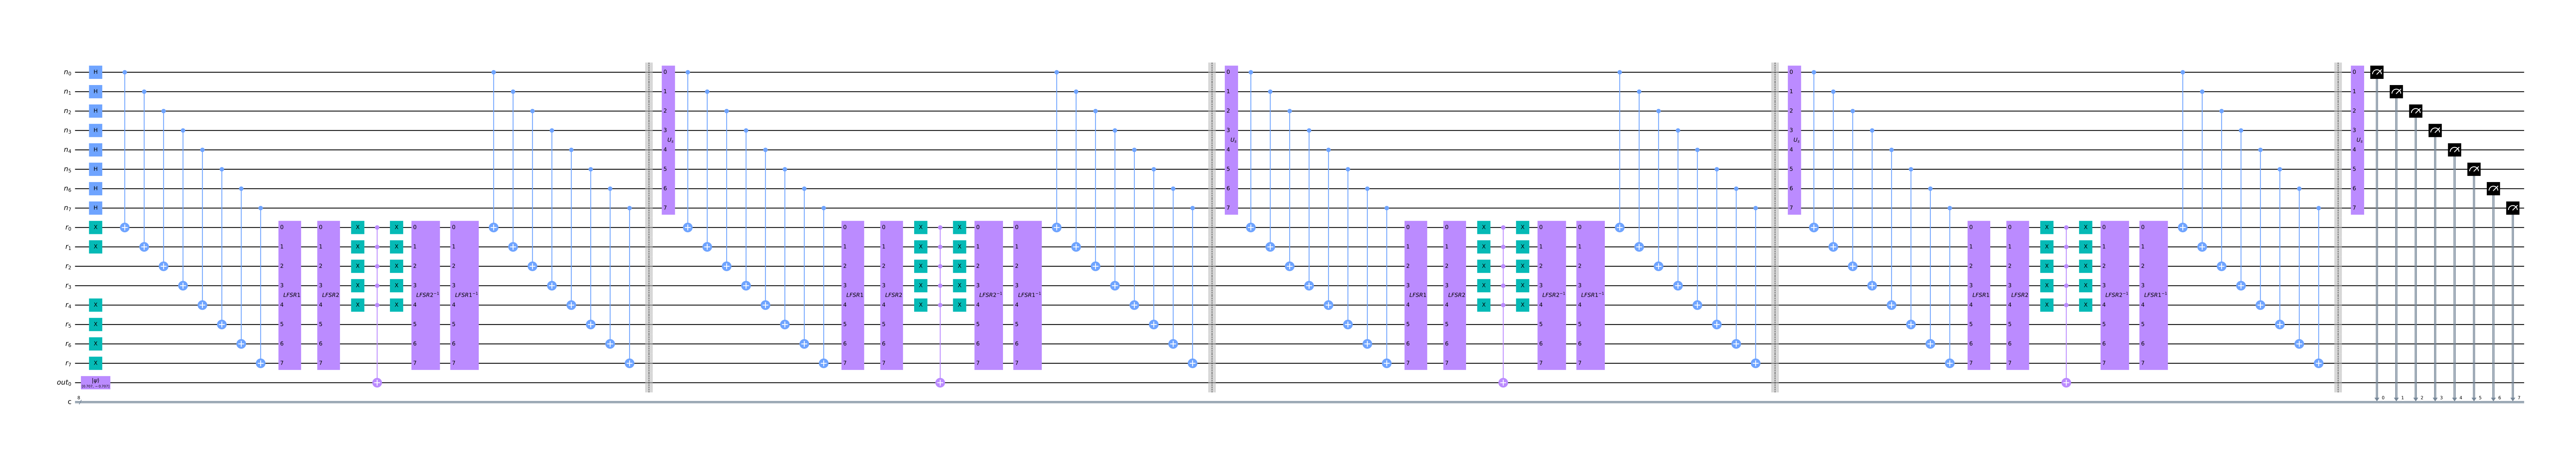
\includegraphics[width=\linewidth]{fig06.09.png}
     \caption{Grover Search Circuit}
     \label{Fig:6.9}
   \end{minipage}
\end{figure}

\subsubsection*{Generalized Grover Search}
Here, we replace the $H$ gate followed by $X$ gate by a single unitary gate. $R_y\left(\bfrac{\pi}{2}\right)$ is a suitable unitary transformation substitute for $HX$. Its inverse is $R_y\left(-\bfrac{\pi}{2}\right)$. We can then simplify our diffuser to the one given in figure \ref{Fig:6.10} thereby reducing 16 gates per iteration.
\begin{figure}[!htb]
   \begin{minipage}{\textwidth}
     \centering
     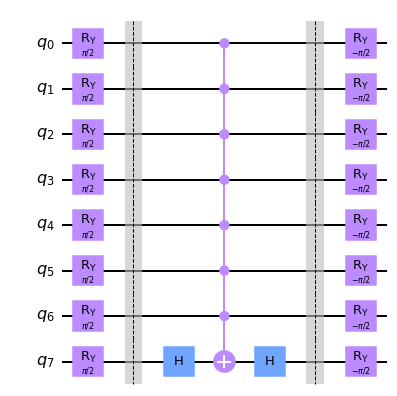
\includegraphics[scale=0.6]{fig06.10.png}
     \caption{Generalised Grover Diffuser}
     \label{Fig:6.10}
   \end{minipage}
\end{figure}
This reduction in the number of gates is very helpful. We will do an analysis of the same in the next section.

